\section{Spiking Neural Networks}

Brief description of what a spiking NN is.

Short summary of how there are many different action potential based units in
the nervous system, but not all units spike.

\section{Hodgkin–Huxley model}

Hodgkin–Huxley models are morphologically and biophysically realistic
representations of Neurons and other spiking components in mammalian nervous
systems \autocite{hodgkin_quantitative_1952}.

\begin{quote}
     Their strength lies in their capacity to map between multiple observables: morphology, electrophysiology, intracellular calcium concentration, and levels of expression and patterns of distributions of ionic currents. Although adding complexity to a model may increase the ability of that model to recreate certain behaviour, finding the right parameters for complex models becomes a challenge\autocite{prinz_alternative_2003}. Furthermore, the computational power needed to simulate sophisticated neural models can be quite large\autocite{markram_reconstruction_2015}.
\end{quote}  

\begin{figure}
    \centering
    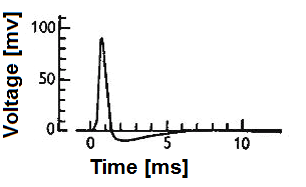
\includegraphics{figures/graphs/huxhog_spike.png}
    \DoubleCaption{The typical form of a neuronal action potential}
    {\small{Source: Nir.nossenson@wikipedia.com, 
        \href{https://creativecommons.org/licenses/by-sa/4.0/deed.en}{CC BY-SA 4.0}}}
    \label{neuronalactionpotentialexample}
\end{figure}

Description of figure \ref{neuronalactionpotentialexample}.

\section{Neuron models for large scale computation}

While it can be desirable to accurately model and simulate the chemical
interactions between individual components of the nervous system, it is
computationally infeasible to do so on a scale similar to that of real-world
system[CITE]. Fortunately, as a network becomes larger, the exact mechanisms of
its individual components can be approximated, and faster activation functions
that perform similarly to real ones can be substituted. 

One such example of a simple model of a spiking neuron is the Leaky Integrate
and Fire (LIF) neuron. It uses BLAH to approximate the action potential spike of
a Hodgkin–Huxley neuron[CITE]. As this is a relatively simple approximation, it
is tempting to assume that such a model would prove inaccurate for anything more
than basic prototypes, however LIF models have been shown to replicate spiking
patterns of more complex models with a low margin of error, provided the models
are under similar naturalistic conditions \autocite{teeter_generalized_2018}.
